%% polyomino.tex
%% Copyright 2024 Matthias Floré
%
% This work may be distributed and/or modified under the
% conditions of the LaTeX Project Public License, either version 1.3c
% of this license or (at your option) any later version.
% The latest version of this license is in
%   http://www.latex-project.org/lppl.txt
% and version 1.3c or later is part of all distributions of LaTeX
% version 2005/12/01 or later.
%
% This work has the LPPL maintenance status `maintained'.
% 
% The Current Maintainer of this work is Matthias Floré.
%
% This work consists of the files polyomino.pdf, polyomino.sty,
% polyomino.tex and README.md.
\documentclass[a4paper,english,dvipsnames]{ltxdoc}
\usepackage[english]{babel}
\usepackage{graphicx}
\usepackage[a4paper,left=2.25cm,right=2.25cm,top=2.5cm,bottom=2.5cm,nohead]{geometry}
\usepackage{parskip}
\usepackage{iftex}
\ifluatex
\else
\usepackage[T1]{fontenc}
\usepackage[utf8]{inputenc}
\fi
\usepackage{mathtools}
\usepackage{amssymb}
\allowdisplaybreaks
\usepackage{pdflscape}
\usepackage{polyomino}
\input{pgfmanual-en-macros.tex}
\usepackage{codehigh}
\usepackage{fancyhdr}
\pagestyle{fancy}
\renewcommand{\headrulewidth}{0pt}
\fancyhead{}
\ExplSyntaxOn
\NewExpandableDocumentCommand \repeatnumber {}
  { \prg_replicate:nn { \thepage } { * } }
\ExplSyntaxOff
\fancyfoot[C]{\IfRefUndefinedExpandable{Thesourcecode}{}{\begin{tikzpicture}[scale=0.9]
\polyomino[
  grid,
  p={*}{style={teal,draw=black}}
]{\repeatnumber}
\end{tikzpicture}}}
\usepackage[nottoc]{tocbibind}
\usepackage{imakeidx}
\makeindex[program=makeindex,columns=2,intoc=true]
\indexsetup{othercode={\thispagestyle{fancy}}}
\AtEndPreamble{\hypersetup{%
linktoc=all,
pdfstartview=FitH,
colorlinks=true,
linkcolor=Mahogany,
citecolor=ForestGreen,
urlcolor=MidnightBlue,
bookmarksnumbered=true,
pdftitle={The polyomino package},
pdfauthor={Matthias Floré},
pdfsubject={Manual},
pdfkeywords={polyomino}}}
\setcounter{tocdepth}{2}
\setcounter{secnumdepth}{2}
\title{The \texttt{polyomino} package\\[12pt]\large Polyominoes using \tikzname{} and \LaTeX3}
\author{Matthias Floré}
\date{Version 1.0 (2024/08/01)}%\\[12pt]
\begin{document}
\maketitle
\thispagestyle{fancy}
\begin{abstract}
\noindent This package is based on the package |tikz| (see \cite{TtTaPGFp}) and can be used to draw polyominoes. It is possible to define custom styles, pics and grids.% This is the manual for version .
\end{abstract}
\tableofcontents
\section{Usage}
The package |polyomino| can be used by putting the following in the preamble.
\begin{codeexample}[code only]
\usepackage{polyomino}
\end{codeexample}
The package |polyomino| loads the package |tikz|.
\section{The command \textbackslash polyomino}
\begin{command}{\polyomino\opt{\oarg{options}}\marg{polyomino specification}}
This command can be placed inside a |tikzpicture| environment. The \meta{polyomino specification} is a token list. Spaces in this list are ignored. With the initial settings, a |,| starts a new row. Otherwise each element in this list corresponds to a cell. An element can consist of multiple characters by surrounding it with braces. The \meta{options} can be given with the keys described in Section \ref{Keys}.
\begin{codeexample}[width=8cm]
\pgfkeys{
  /polyomino,
  p={F}{style={blue,draw=black,ultra thick}},
  p={I}{style={brown,draw=black,ultra thick}},
  p={L}{style={cyan,draw=black,ultra thick}},
  p={N}{style={gray,draw=black,ultra thick}},
  p={P}{style={lime,draw=black,ultra thick}},
  p={T}{style={magenta,draw=black,ultra thick}},
  p={U}{style={olive,draw=black,ultra thick}},
  p={V}{style={orange,draw=black,ultra thick}},
  p={W}{style={pink,draw=black,ultra thick}},
  p={X}{style={purple,draw=black,ultra thick}},
  p={Y}{style={red,draw=black,ultra thick}},
  p={Z}{style={teal,draw=black,ultra thick}}
}
\begin{tikzpicture}
\polyomino[
  grid
]{
  UUUVVV,
  UXUZZV,
  XXXFZV,
  IXFFZZ,
  ILLFFT,
  ILNTTT,
  ILNWWT,
  ILNNWW,
  PPPNYW,
  PPYYYY
}
\end{tikzpicture}
\end{codeexample}
The algorithm constructs the border of each polyomino. It does not consider holes determined by empty cells. Although it does detect a cell inside a polyomino which has a different style. This is illustrated in the example below.
\begin{codeexample}[width=10cm]
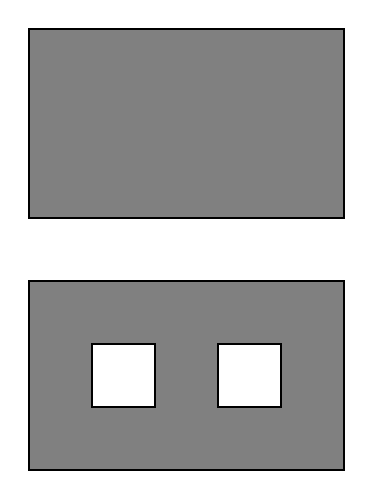
\begin{tikzpicture}[scale=0.8]
\polyomino[
  p={a}{style={gray,draw=black,thick}}
]{
  aaaaa,
  a.a.a,
  aaaaa
}
\polyomino[
  at={(0,-4)},
  p={a}{style={gray,draw=black,thick}},
  p={*}{style={white,draw=black,thick}}
]{
  aaaaa,
  a*a*a,
  aaaaa
}
\end{tikzpicture}
\end{codeexample}
\end{command}
\section{Keys}\label{Keys}
The keys in this Section can be given as \meta{options} to the command |\polyomino|.

There are two key families: |/polyomino| and |/polyomino/p_2|. The key family |/polyomino| is intended for usage in documents whereas |/polyomino/p_2| is not. In the key family |/polyomino|, also keys from the key family |/polyomino/p_2| will be looked up. The second argument from the key |p| only accepts keys from the key family |/polyomino/p_2|.
\begin{key}{/polyomino/at=\marg{point} (initially (0,0))}
This key defines the bottom left coordinate of the polyomino.
\end{key}
\begin{key}{/polyomino/p\_2/connected}
This key sets the |pic| type (which is activated by the key |pic|) to false. This is the initial setting.
\end{key}
\begin{key}{/polyomino/p\_2/discrete}
This key sets the |pic| type (which is activated by the key |pic|) to true.
\end{key}
\begin{key}{/polyomino/empty cell=\marg{token list} (initially .)}
A cell corresponding to the \meta{token list} in the \meta{polyomino specification} will be left empty.

A cell corresponding to the empty token list will always be left empty.
\end{key}
\begin{key}{/polyomino/grid=\opt{\meta{boolean}} (default true, initially false)}
If true then a grid is drawn. The grid does not apply to borders of polyominoes. The style of this grid is determined by the key |grid style|. A grid does not apply to a cell with a |pic|.
\end{key}
\begin{stylekey}{/polyomino/grid style=\marg{options} (initially \normalfont empty)}
This key determines the style of the grid.
\begin{codeexample}[width=6.5cm]
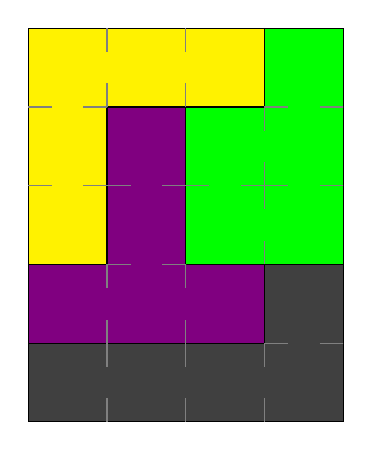
\begin{tikzpicture}[rotate=90]
\polyomino[
  grid,
  grid style={gray,dash pattern=on 3mm off 4mm on 3mm off 0mm},
  p={L}{style={darkgray,draw=black}},
  p={P}{style={green,draw=black}},
  p={T}{style={violet,draw=black}},
  p={V}{style={yellow,draw=black}}
]{
  LTVVV,
  LTTTV,
  LTPPV,
  LLPPP
}
\end{tikzpicture}
\end{codeexample}
\end{stylekey}
\begin{stylekey}{/polyomino/p\_2/p=\marg{name}\marg{options} (initially \normalfont empty)}
This key determines the style of the polyomino with \meta{name} in the \meta{polyomino specification}.

The \meta{options} only accept keys from the key family |/polyomino/p_2|.

In the example below, the polyominoes have the same shape but are differentiated by using different names.
\begin{codeexample}[width=10cm]
\begin{tikzpicture}
\pgfkeys{
  /polyomino,
  p={a}{},
  p={b}{},
  style={fill=none,draw}
}
\def\example{
  aa,
  ab,
  ab,
  bb
}
\polyomino{\example}
\polyomino[
  at={(2,0)}
]{\example}
\end{tikzpicture}
\end{codeexample}
\end{stylekey}
\begin{key}{/polyomino/p\_2/pic=\marg{code}}
The \meta{code} defines the |pic| which is used for each cell of the polyomino.

A grid does not apply to a cell with a |pic|.
\begin{codeexample}[width=7cm]
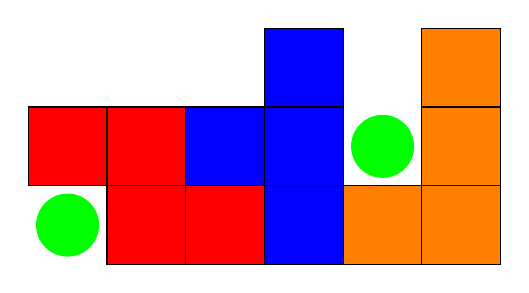
\begin{tikzpicture}
\polyomino[
  empty cell=*,
  grid,
  p={a}{style={red,draw=black}},
  p={b}{style={blue,draw=black}},
  p={c}{style={orange,draw=black}},
  p={circle}{pic={\fill[green] (0,0) circle[radius=0.4];}},
  row sep=;
]{
     {}    * * b    {}    c ;
     a     a b b {circle} c ;
  {circle} a a b    c     c
}
\end{tikzpicture}
\end{codeexample}
\begin{codeexample}[width=5cm]
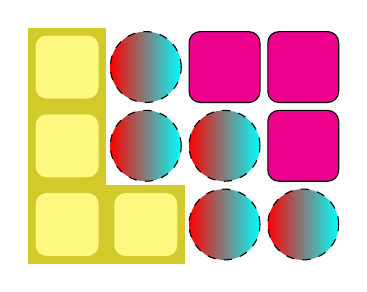
\begin{tikzpicture}
\polyomino[
  p={circle}{
    pic={\path[pic actions] (0,0) circle[radius=0.45];},
    style={right color=cyan,left color=red,draw,dashed}
  },
  p={L}{
    pic={
      \fill[yellow!80!black] (-0.5,-0.5) rectangle +(1,1);
      \fill[yellow!50,rounded corners] (-0.4,-0.4) rectangle +(0.8,0.8);
    }
  },
  p={square}{
    pic={\path[pic actions] (-0.45,-0.45) rectangle +(0.9,0.9);},
    style={fill=magenta,draw,rounded corners}
  }
]{
  L {circle} {square} {square} ,
  L {circle} {circle} {square} ,
  L    L     {circle} {circle}
}
\end{tikzpicture}
\end{codeexample}
\end{key}
\begin{key}{/polyomino/row sep=\marg{token list} (initially ,)}
The \meta{token list} in the \meta{polyomino specification} will start a new row.
\end{key}
\begin{stylekey}{/polyomino/p\_2/style=\marg{options} (initially \normalfont empty)}
This key determines the style of the polyomino.
\end{stylekey}
\begin{thebibliography}{9}
\bibitem{TtTaPGFp}
Till Tantau,
\emph{The \tikzname{} and {\upshape\pgfname} Packages},
Manual for version 3.1.10,
\url{https://ctan.org/pkg/pgf},
2023.
\end{thebibliography}
\printindex
\newgeometry{left=2.25cm,right=2.25cm,top=2.25cm,bottom=2.25cm}
\pagestyle{plain}
\appendix
\begin{landscape}
\section{The source code}\label{Thesourcecode}
\dochighinput[language=latex/latex3]{polyomino.sty}
\end{landscape}
\end{document}